\documentclass[12pt,a4paper]{article}

% ===== PACKAGES =====
\usepackage[utf8]{inputenc}
\usepackage[T1]{fontenc}
\usepackage{lmodern}
\usepackage[margin=2cm]{geometry}
\usepackage{hyperref}
\usepackage{xcolor}
\usepackage{listings}
\usepackage{booktabs}
\usepackage{enumitem}
\usepackage{titlesec}
\usepackage{fancyhdr}
\usepackage{graphicx}
\usepackage{tcolorbox}
\usepackage{array}
\usepackage{longtable}
\usepackage{tikz}
\usetikzlibrary{shapes.geometric, arrows.meta, positioning}

% ===== COLORS =====
\definecolor{primaryblue}{HTML}{1A5276}
\definecolor{secondaryblue}{HTML}{2980B9}
\definecolor{accentgreen}{HTML}{27AE60}
\definecolor{codebg}{HTML}{F4F4F4}
\definecolor{darkgray}{HTML}{2C3E50}
\definecolor{answerbox}{HTML}{EBF5FB}
\definecolor{tipbox}{HTML}{EAFAF1}
\definecolor{warnbox}{HTML}{FEF9E7}

% ===== HYPERREF SETUP =====
\hypersetup{
    colorlinks=true,
    linkcolor=primaryblue,
    urlcolor=secondaryblue
}

% ===== CODE LISTING SETUP =====
\lstset{
    backgroundcolor=\color{codebg},
    basicstyle=\ttfamily\small,
    breaklines=true,
    frame=single,
    rulecolor=\color{gray!40},
    tabsize=4,
    showstringspaces=false,
    keywordstyle=\color{primaryblue}\bfseries,
    commentstyle=\color{accentgreen},
    stringstyle=\color{red!70!black},
}

\lstdefinelanguage{JavaCustom}{
    language=Java,
    morekeywords={var, record, String},
}

% ===== TCOLORBOX STYLES =====
\tcbuselibrary{skins, breakable}

\newtcolorbox{answerbox}{
    colback=answerbox,
    colframe=secondaryblue,
    fonttitle=\bfseries,
    title=Answer,
    breakable,
    left=5pt, right=5pt, top=5pt, bottom=5pt
}

\newtcolorbox{tipbox}{
    colback=tipbox,
    colframe=accentgreen,
    fonttitle=\bfseries,
    title={Pro Tip},
    breakable,
    left=5pt, right=5pt, top=5pt, bottom=5pt
}

\newtcolorbox{warnbox}{
    colback=warnbox,
    colframe=orange!80!black,
    fonttitle=\bfseries,
    title={Important},
    breakable,
    left=5pt, right=5pt, top=5pt, bottom=5pt
}

% ===== SECTION FORMATTING =====
\titleformat{\section}
  {\color{primaryblue}\Large\bfseries}
  {\thesection.}{0.5em}{}[\color{primaryblue}\titlerule]

\titleformat{\subsection}
  {\color{secondaryblue}\large\bfseries}
  {Q\thesubsection.}{0.5em}{}

% ===== HEADER / FOOTER =====
\pagestyle{fancy}
\fancyhf{}
\fancyhead[L]{\textcolor{primaryblue}{\textbf{Education CRM Project --- Interview Guide}}}
\fancyhead[R]{\textcolor{gray}{\thepage}}
\fancyfoot[C]{\textcolor{gray}{\small Prepared for Java Full-Stack Spring Boot Interview}}
\renewcommand{\headrulewidth}{1pt}
\renewcommand{\headrule}{\hbox to\headwidth{\color{primaryblue}\leaders\hrule height \headrulewidth\hfill}}

% ===== DOCUMENT START =====
\begin{document}

% ===== TITLE PAGE =====
\begin{titlepage}
\centering
\vspace*{3cm}

{\Huge\bfseries\color{primaryblue} Education CRM Project\\[0.3cm]}
{\LARGE\color{secondaryblue} Complete Interview Guide\\[0.5cm]}
{\Large Java Full-Stack $\mid$ Spring Boot $\mid$ Thymeleaf $\mid$ MySQL\\[2cm]}

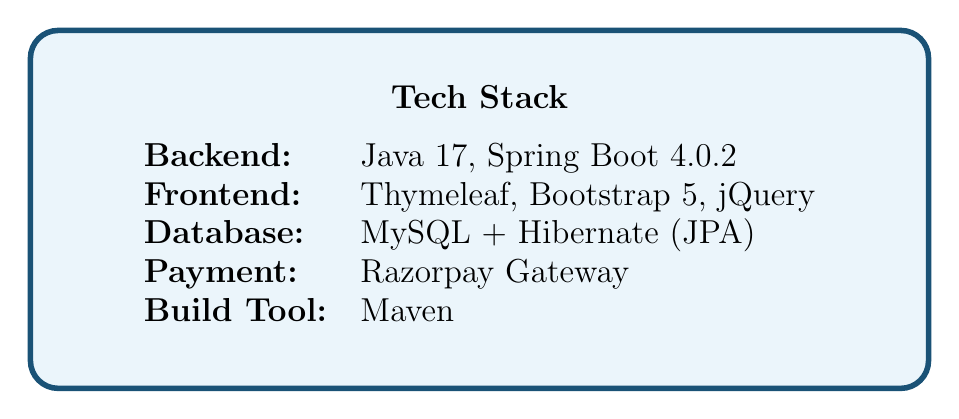
\begin{tikzpicture}
\node[draw=primaryblue, line width=2pt, rounded corners=10pt, inner sep=20pt, fill=answerbox] {
    \begin{minipage}{10cm}
    \centering
    \large\textbf{Tech Stack}\\[10pt]
    \begin{tabular}{ll}
    \textbf{Backend:} & Java 17, Spring Boot 4.0.2 \\
    \textbf{Frontend:} & Thymeleaf, Bootstrap 5, jQuery \\
    \textbf{Database:} & MySQL + Hibernate (JPA) \\
    \textbf{Payment:} & Razorpay Gateway \\
    \textbf{Build Tool:} & Maven \\
    \end{tabular}
    \end{minipage}
};
\end{tikzpicture}

\vfill
{\large\color{darkgray} \today}
\end{titlepage}

% ===== TABLE OF CONTENTS =====
\tableofcontents
\newpage

% ======================================================================
\section{Project Introduction}
% ======================================================================

\begin{answerbox}
``I developed an \textbf{Education CRM (Customer Relationship Management)} web application using \textbf{Spring Boot} as the backend framework and \textbf{Thymeleaf} as the server-side template engine. The application allows students to \textbf{register, login, browse courses, and purchase courses online} using the \textbf{Razorpay payment gateway}. The project follows the \textbf{MVC (Model-View-Controller) architecture} with a 3-layer design --- Controller, Service, and Repository layer.''
\end{answerbox}

\subsection*{Technology Stack}

\begin{center}
\begin{tabular}{>{\bfseries}l l}
\toprule
\textbf{Layer} & \textbf{Technology} \\
\midrule
Backend        & Java 17, Spring Boot 4.0.2 \\
Frontend       & Thymeleaf, HTML5, Bootstrap 5, jQuery \\
Database       & MySQL (via Spring Data JPA + Hibernate) \\
Payment        & Razorpay Payment Gateway \\
Build Tool     & Maven \\
Validation     & Jakarta Bean Validation (\texttt{@Valid}, \texttt{@Pattern}) \\
Session Mgmt   & Spring \texttt{@SessionAttributes} \\
\bottomrule
\end{tabular}
\end{center}

% ======================================================================
\section{Project Architecture \& Flow}
% ======================================================================

\begin{center}
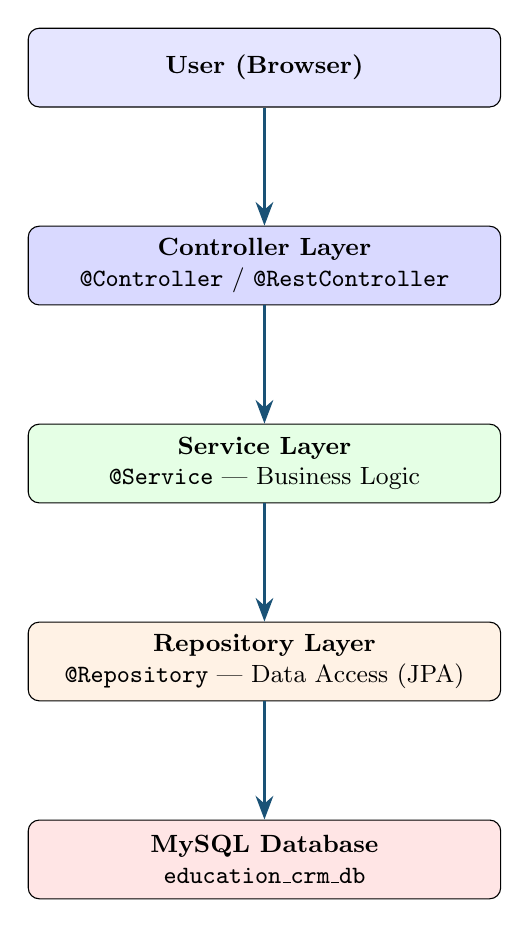
\begin{tikzpicture}[
    node distance=1.5cm,
    every node/.style={draw, rounded corners, minimum width=6cm, minimum height=1cm, align=center, font=\small},
    arrow/.style={-{Stealth[length=3mm]}, thick, color=primaryblue}
]
\node (browser) [fill=blue!10] {\textbf{User (Browser)}};
\node (controller) [below=of browser, fill=blue!15] {\textbf{Controller Layer} \\ \texttt{@Controller} / \texttt{@RestController}};
\node (service) [below=of controller, fill=green!10] {\textbf{Service Layer} \\ \texttt{@Service} --- Business Logic};
\node (repo) [below=of service, fill=orange!10] {\textbf{Repository Layer} \\ \texttt{@Repository} --- Data Access (JPA)};
\node (db) [below=of repo, fill=red!10] {\textbf{MySQL Database} \\ \texttt{education\_crm\_db}};

\draw[arrow] (browser) -- (controller);
\draw[arrow] (controller) -- (service);
\draw[arrow] (service) -- (repo);
\draw[arrow] (repo) -- (db);
\end{tikzpicture}
\end{center}

\subsection*{3 Entity Classes (Database Tables)}

\begin{enumerate}
    \item \textbf{User} --- \texttt{id, name, email, password, phoneno, city}
    \item \textbf{Course} --- \texttt{id, name, description, originalPrice, discountedPrice, updatedOn, imageUrl}
    \item \textbf{Orders} --- \texttt{id, courseName, courseAmount, userEmail, orderId, dateOfPurchase, rzpPaymentId}
\end{enumerate}

% ======================================================================
\section{Feature-Wise Interview Questions}
% ======================================================================

\setcounter{subsection}{0}

% ---------- Q1 ----------
\subsection{Project ke features kya hain?}

\begin{answerbox}
\begin{enumerate}
    \item \textbf{User Registration} with server-side + client-side validation
    \item \textbf{User Login/Logout} with session management
    \item \textbf{Course Listing} --- dynamic courses fetched from MySQL database
    \item \textbf{Razorpay Payment Integration} --- real-time online payment
    \item \textbf{Order Storage} --- payment details stored in Orders table
    \item \textbf{Dynamic Header} --- different navbar for logged-in vs guest users (Thymeleaf fragments)
    \item \textbf{Profile Page} --- shows logged-in user details from session
\end{enumerate}
\end{answerbox}

% ---------- Q2 ----------
\subsection{MVC architecture kaise implement kiya?}

\begin{answerbox}
\begin{itemize}
    \item \textbf{Model} --- Entity classes (\texttt{User}, \texttt{Course}, \texttt{Orders}) mapped to database tables using JPA annotations (\texttt{@Entity}, \texttt{@Id}, \texttt{@GeneratedValue}, \texttt{@Column})
    \item \textbf{View} --- Thymeleaf HTML templates (\texttt{index.html}, \texttt{login.html}, \texttt{register.html}, \texttt{user-profile.html})
    \item \textbf{Controller} --- \texttt{UserController} handles web requests (\texttt{@GetMapping}, \texttt{@PostMapping}); \texttt{OrdersApi} handles REST API calls (\texttt{@RestController})
\end{itemize}
\end{answerbox}

% ---------- Q3 ----------
\subsection{\texttt{@SpringBootApplication} kya karta hai?}

\begin{answerbox}
Yeh 3 annotations ka combination hai:
\begin{enumerate}
    \item \texttt{@Configuration} --- marks class as a source of bean definitions
    \item \texttt{@EnableAutoConfiguration} --- Spring Boot automatically configures beans based on classpath dependencies
    \item \texttt{@ComponentScan} --- scans \texttt{in.gw.main} package and sub-packages for \texttt{@Controller}, \texttt{@Service}, \texttt{@Repository} components
\end{enumerate}
\end{answerbox}

% ---------- Q4 ----------
\subsection{\texttt{@Controller} vs \texttt{@RestController} mein kya difference hai?}

\begin{answerbox}
\begin{itemize}
    \item \texttt{@Controller} --- returns \textbf{view name} (HTML page). \texttt{UserController} mein use kiya kyunki woh Thymeleaf pages return karta hai (\texttt{return "login"}, \texttt{return "register"})
    \item \texttt{@RestController} --- returns \textbf{data directly} (JSON/text). \texttt{@Controller + @ResponseBody} ka shortcut hai. \texttt{OrdersApi} mein use kiya kyunki woh AJAX call se data accept karta hai aur \texttt{ResponseEntity<String>} return karta hai --- no view, only data.
\end{itemize}
\end{answerbox}

% ---------- Q5 ----------
\subsection{\texttt{@SessionAttributes("sessionUser")} kaise kaam karta hai?}

\begin{answerbox}
\begin{itemize}
    \item Jab user login karta hai, \texttt{model.addAttribute("sessionUser", authenticatedUser)} se user object session mein store hota hai
    \item Yeh session tab tak active rehta hai jab tak \texttt{sessionStatus.setComplete()} call na ho (logout pe)
    \item Har page pe \texttt{\$\{sessionUser.name\}}, \texttt{\$\{sessionUser.email\}} se user info dikhate hain
    \item Agar \texttt{sessionUser == null} hai toh guest header dikhta hai, warna logged-in user header
\end{itemize}
\end{answerbox}

% ---------- Q6 ----------
\subsection{Login flow explain karo step by step}

\begin{answerbox}
\begin{enumerate}
    \item User opens \texttt{/login} $\rightarrow$ \texttt{UserController.openLoginPage()} $\rightarrow$ returns \texttt{login.html} with empty \texttt{User} object
    \item User fills email + password $\rightarrow$ form POSTs to \texttt{/loginform}
    \item \texttt{handleLoginForm()} calls \texttt{userService.loginUserService(email, password)}
    \item Service layer calls \texttt{userRepository.findByEmail(email)} --- yeh \textbf{derived query method} hai
    \item Agar user milta hai aur password match karta hai $\rightarrow$ \texttt{return true}
    \item Controller mein authenticated user ko session mein store karta hai via \texttt{model.addAttribute("sessionUser", authenticatedUser)}
    \item Returns \texttt{user-profile} view
\end{enumerate}
\end{answerbox}

% ---------- Q7 ----------
\subsection{\texttt{findByEmail(String email)} --- yeh query nahi likhi, toh kaise chali?}

\begin{answerbox}
Yeh \textbf{Spring Data JPA Derived Query Method} hai. Spring Data JPA method ka naam parse karta hai:
\begin{itemize}
    \item \texttt{findBy} $\rightarrow$ SELECT query
    \item \texttt{Email} $\rightarrow$ WHERE clause on \texttt{email} column
\end{itemize}
Internally yeh generate karta hai:
\begin{lstlisting}[language=SQL]
SELECT * FROM user WHERE email = ?
\end{lstlisting}
Humein koi \texttt{@Query} ya native SQL likhne ki zaroorat nahi.
\end{answerbox}

% ---------- Q8 ----------
\subsection{Validation kaise implement kiya?}

\begin{answerbox}
\textbf{Server-side validation} using Jakarta Bean Validation:
\begin{itemize}
    \item \texttt{@Pattern(regexp = "\^{}[a-z,A-Z ]\{5,25\}\$")} on \texttt{name} field --- only letters, 5--25 chars
    \item \texttt{@Pattern} with email regex on \texttt{email} --- validates email format
    \item \texttt{@Pattern(regexp = "\^{}[0-9]\{10\}\$")} on \texttt{phoneno} --- exactly 10 digits
    \item \texttt{@Valid} annotation on controller method parameter triggers validation
    \item \texttt{BindingResult} object captures validation errors
    \item If \texttt{result.hasErrors()} $\rightarrow$ return to same form page with error messages
    \item In Thymeleaf: \texttt{th:if="\$\{\#fields.hasErrors('name')\}"} shows field-specific errors
\end{itemize}

\textbf{Client-side}: \texttt{required} attribute + custom \texttt{onsubmit="return validateForm()"} on register form
\end{answerbox}

% ---------- Q9 ----------
\subsection{Razorpay Payment Integration kaise kiya?}

\begin{answerbox}
\textbf{Frontend (JavaScript):}
\begin{enumerate}
    \item Jab user ``Buy'' button click karta hai, \texttt{purchasecource()} function call hota hai
    \item Course name, amount, user details pass hote hain
    \item Razorpay checkout popup open hota hai with options (key, amount in paisa, currency INR)
    \item Payment success hone pe \texttt{handler} function trigger hota hai
    \item Handler mein AJAX POST call (\texttt{\$.ajax}) jaati hai \texttt{/api/storeOrderDetails} pe with order data
\end{enumerate}

\textbf{Backend (REST API):}
\begin{enumerate}
    \item \texttt{OrdersApi.storeUserOrders()} method receives JSON body
    \item \texttt{RazorpayClient} initialize hota hai with API key + secret
    \item Server-side Razorpay order create hota hai with amount, currency, receipt
    \item Generated \texttt{orderId} set hota hai in Orders entity
    \item \texttt{orderService.storeUserOrders(orders)} $\rightarrow$ \texttt{orderRepository.save(orders)} $\rightarrow$ MySQL mein save
\end{enumerate}
\end{answerbox}

% ---------- Q10 ----------
\subsection{\texttt{@Autowired} kya hai? Kaise kaam karta hai?}

\begin{answerbox}
\begin{itemize}
    \item Yeh \textbf{Dependency Injection} ka mechanism hai
    \item Spring container automatically matching bean dhundh ke inject kar deta hai
    \item Example: \texttt{@Autowired private UserService userService;} $\rightarrow$ Spring apna \texttt{UserService} bean inject karega
    \item Yeh \textbf{Inversion of Control (IoC)} principle follow karta hai --- hum object nahi banate, Spring banata hai
\end{itemize}
\end{answerbox}

% ---------- Q11 ----------
\subsection{JPA annotations explain karo}

\begin{answerbox}
\begin{center}
\begin{tabular}{>{\ttfamily}l p{9cm}}
\toprule
\textbf{Annotation} & \textbf{Purpose} \\
\midrule
@Entity & Marks class as a database table \\
@Id & Marks primary key field \\
@GeneratedValue(strategy = GenerationType.IDENTITY) & Auto-increment primary key (MySQL AI) \\
@Column & Maps field to table column (optional if name matches) \\
\bottomrule
\end{tabular}
\end{center}
\end{answerbox}

% ---------- Q12 ----------
\subsection{\texttt{spring.jpa.hibernate.ddl-auto = update} ka kya matlab hai?}

\begin{answerbox}
\begin{itemize}
    \item \texttt{update} --- Hibernate automatically creates/updates tables based on entity classes. Agar table exist karti hai toh modify karega, nahi hai toh create karega. \textbf{Data delete nahi hota.}
    \item Other options:
    \begin{itemize}
        \item \texttt{create} --- drop + create every time (data loss)
        \item \texttt{create-drop} --- drop on shutdown
        \item \texttt{validate} --- only validates schema, no changes
        \item \texttt{none} --- kuch nahi karega
    \end{itemize}
    \item Production mein \texttt{validate} ya \texttt{none} use karte hain, \texttt{update} sirf development ke liye
\end{itemize}
\end{answerbox}

% ---------- Q13 ----------
\subsection{\texttt{spring.jpa.show-sql = true} kya karta hai?}

\begin{answerbox}
Hibernate ki generated SQL queries console mein print hoti hain --- debugging ke liye useful hai.
\end{answerbox}

% ---------- Q14 ----------
\subsection{Thymeleaf Fragments kyun use kiye?}

\begin{answerbox}
\begin{itemize}
    \item \textbf{Code Reusability} --- Navbar code har page pe likhne ki jagah ek baar \texttt{header.html} aur \texttt{user-header.html} mein likha
    \item \texttt{th:fragment="crm-header"} --- fragment define karna
    \item \texttt{th:replace="\~{}\{fragment/header :: crm-header\}"} --- fragment include karna
    \item \textbf{DRY Principle} (Don't Repeat Yourself) follow kiya
    \item Do alag headers hain:
    \begin{itemize}
        \item \texttt{crm-header} --- guest users ke liye (Login + Register buttons)
        \item \texttt{u-header} --- logged-in users ke liye (Home, My Courses, Profile, Logout)
    \end{itemize}
\end{itemize}
\end{answerbox}

% ---------- Q15 ----------
\subsection{Conditional rendering kaise kiya Thymeleaf mein?}

\begin{answerbox}
\begin{lstlisting}[language=HTML]
<div th:if="${sessionUser == null OR sessionUser == ''}">
    <!-- Guest header -->
</div>
<div th:unless="${sessionUser == null OR sessionUser == ''}">
    <!-- Logged-in user header -->
</div>
\end{lstlisting}
\begin{itemize}
    \item \texttt{th:if} --- condition true hone pe render hoga
    \item \texttt{th:unless} --- condition false hone pe render hoga (opposite of \texttt{th:if})
    \item \texttt{th:each} --- loop ke liye: \texttt{th:each="course : \$\{coursesList\}"} --- courses iterate karne ke liye
\end{itemize}
\end{answerbox}

% ---------- Q16 ----------
\subsection{\texttt{JpaRepository} kya hai aur kyun extend kiya?}

\begin{answerbox}
\begin{itemize}
    \item \texttt{JpaRepository<Entity, ID\_Type>} Spring Data JPA ka interface hai
    \item Yeh \textbf{CRUD operations free mein deta hai} bina code likhe:
    \begin{itemize}
        \item \texttt{save()} --- INSERT / UPDATE
        \item \texttt{findAll()} --- SELECT *
        \item \texttt{findById()} --- SELECT WHERE id = ?
        \item \texttt{deleteById()} --- DELETE WHERE id = ?
        \item \texttt{count()} --- COUNT(*)
    \end{itemize}
    \item Hierarchy: \texttt{JpaRepository} $\rightarrow$ \texttt{PagingAndSortingRepository} $\rightarrow$ \texttt{CrudRepository} $\rightarrow$ \texttt{Repository}
\end{itemize}
\end{answerbox}

% ---------- Q17 ----------
\subsection{\texttt{@Service} annotation ka kya role hai?}

\begin{answerbox}
\begin{itemize}
    \item Business logic layer ko mark karta hai
    \item Spring component scan mein include hota hai --- IoC container mein bean ban jaata hai
    \item \textbf{Why separate Service layer?}
    \begin{itemize}
        \item Controller sirf request handle kare
        \item Service mein business logic ho (login check, data processing)
        \item Repository sirf database operations kare
        \item \textbf{Separation of Concerns} principle
    \end{itemize}
\end{itemize}
\end{answerbox}

% ---------- Q18 ----------
\subsection{Exception handling kaise kiya registration mein?}

\begin{answerbox}
\begin{lstlisting}[language=JavaCustom]
try {
    userService.registerUserService(user);
    model.addAttribute("successmsg", "Registered Successfully");
    return "register";
} catch(Exception e) {
    e.printStackTrace();
    model.addAttribute("errormsg", "Registration Failed");
    return "error";
}
\end{lstlisting}
Try-catch se database errors (duplicate email, connection failure) handle hote hain. Success pe green alert dikhta hai, failure pe error page.
\end{answerbox}

% ---------- Q19 ----------
\subsection{Password plain text mein store kar rahe ho --- iska kya issue hai?}

\begin{tipbox}
\textit{(Interviewer impress hoga agar khud se bolo)}\\[5pt]
``Currently password plain text mein stored hai. Production mein \textbf{BCryptPasswordEncoder} use karna chahiye jo password ko hash karta hai. Spring Security ka \texttt{PasswordEncoder} interface use karke hum one-way hashing implement kar sakte hain jisse password database mein readable form mein kabhi na rahe.''
\end{tipbox}

% ---------- Q20 ----------
\subsection{Agar Spring Security add karna ho toh kya karoge?}

\begin{answerbox}
\begin{enumerate}
    \item \texttt{spring-boot-starter-security} dependency add karenge
    \item \texttt{SecurityConfig} class banayenge with \texttt{@EnableWebSecurity}
    \item \texttt{SecurityFilterChain} bean mein URL authorization configure karenge --- kaunse URLs public hain, kaunse authenticated users ke liye
    \item \texttt{BCryptPasswordEncoder} bean add karenge for password hashing
    \item \texttt{UserDetailsService} implement karenge --- custom login logic with hashed password comparison
    \item Session management Spring Security handle karega automatically
\end{enumerate}
\end{answerbox}

% ======================================================================
\section{General Spring Boot Interview Questions}
% ======================================================================

\setcounter{subsection}{20}

% ---------- Q21 ----------
\subsection{Spring Boot ke advantages kya hain?}

\begin{answerbox}
\begin{enumerate}
    \item \textbf{Auto Configuration} --- dependencies ke basis pe automatically configure karta hai
    \item \textbf{Embedded Server} --- Tomcat embedded hai, alag se server install nahi karna
    \item \textbf{Starter Dependencies} --- \texttt{spring-boot-starter-web} add karo, sab related dependencies aa jayengi
    \item \textbf{Production Ready} --- Actuator, health checks, metrics
    \item \textbf{Rapid Development} --- kam boilerplate code
\end{enumerate}
\end{answerbox}

% ---------- Q22 ----------
\subsection{\texttt{application.properties} mein kya configure kiya?}

\begin{answerbox}
\begin{enumerate}
    \item \textbf{Database URL} --- \texttt{jdbc:mysql://localhost:3306/education\_crm\_db}
    \item \textbf{DB credentials} --- username, password
    \item \textbf{Hibernate DDL auto} --- \texttt{update} (auto table creation)
    \item \textbf{Show SQL} --- \texttt{true} (debugging)
\end{enumerate}
\end{answerbox}

% ---------- Q23 ----------
\subsection{Maven kya hai? \texttt{pom.xml} mein kya hota hai?}

\begin{answerbox}
Maven ek \textbf{build tool} hai --- dependency management, build, packaging karta hai.\\[5pt]
\texttt{pom.xml} mein:
\begin{itemize}
    \item \textbf{Parent} --- \texttt{spring-boot-starter-parent} (version management)
    \item \textbf{Dependencies} --- JPA, MySQL, Thymeleaf, Web, Validation, Razorpay
    \item \textbf{Properties} --- Java version 17
    \item \textbf{Plugins} --- Spring Boot Maven Plugin
\end{itemize}
\end{answerbox}

% ---------- Q24 ----------
\subsection{\texttt{@ModelAttribute} kya karta hai?}

\begin{answerbox}
\begin{itemize}
    \item Form data ko Java object mein bind karta hai
    \item \texttt{@ModelAttribute("user") User user} --- form fields automatically \texttt{User} object ke fields mein map hote hain
    \item Name, email, password, phoneno, city $\rightarrow$ sab auto-populate
\end{itemize}
\end{answerbox}

% ---------- Q25 ----------
\subsection{\texttt{ResponseEntity} kya hai?}

\begin{answerbox}
\begin{itemize}
    \item Full HTTP response ko represent karta hai --- body + headers + status code
    \item \texttt{ResponseEntity.ok("Order Details Stored Successfully")} $\rightarrow$ 200 OK status with message body
    \item REST API mein use hota hai proper HTTP response bhejne ke liye
\end{itemize}
\end{answerbox}

% ---------- Q26 ----------
\subsection{\texttt{@RequestBody} vs \texttt{@ModelAttribute} mein kya difference hai?}

\begin{answerbox}
\begin{center}
\begin{tabular}{p{6cm} p{6cm}}
\toprule
\textbf{\texttt{@RequestBody}} & \textbf{\texttt{@ModelAttribute}} \\
\midrule
JSON data accept karta hai & Form data accept karta hai \\
AJAX / REST calls ke liye & HTML form submissions ke liye \\
Content-Type: application/json & Content-Type: form-urlencoded \\
\texttt{OrdersApi} mein use kiya & \texttt{UserController} mein use kiya \\
\bottomrule
\end{tabular}
\end{center}
\end{answerbox}

% ---------- Q27 ----------
\subsection{Thymeleaf ke important attributes kaunse use kiye?}

\begin{answerbox}
\begin{center}
\begin{tabular}{>{\ttfamily}l l}
\toprule
\textbf{Attribute} & \textbf{Use} \\
\midrule
th:text="\$\{...\}" & Dynamic text display \\
th:each="item : \$\{list\}" & Looping (for-each) \\
th:if / th:unless & Conditional rendering \\
th:field="*\{name\}" & Form field binding \\
th:object="\$\{user\}" & Form object binding \\
th:src="@\{\$\{url\}\}" & Dynamic image URL \\
th:replace="\~{}\{...\}" & Fragment inclusion \\
th:data-* & Custom data attributes \\
\bottomrule
\end{tabular}
\end{center}
\end{answerbox}

% ---------- Q28 ----------
\subsection{Project mein kaunsa design pattern use kiya?}

\begin{answerbox}
\begin{enumerate}
    \item \textbf{MVC Pattern} --- Controller-Service-Repository separation
    \item \textbf{Repository Pattern} --- JpaRepository for data access abstraction
    \item \textbf{Template Method Pattern} --- Thymeleaf fragments for reusable UI
    \item \textbf{Dependency Injection} --- \texttt{@Autowired} for loose coupling
    \item \textbf{Singleton Pattern} --- Spring beans are singleton by default
\end{enumerate}
\end{answerbox}

% ---------- Q29 ----------
\subsection{\texttt{@GetMapping} vs \texttt{@PostMapping} kab use kiya?}

\begin{answerbox}
\begin{center}
\begin{tabular}{p{6cm} p{6cm}}
\toprule
\textbf{\texttt{@GetMapping}} & \textbf{\texttt{@PostMapping}} \\
\midrule
Data \textbf{fetch/display} karne ke liye & Data \textbf{submit} karne ke liye \\
\texttt{/index}, \texttt{/login}, \texttt{/register}, \texttt{/logout} & \texttt{/loginform}, \texttt{/regform} \\
Idempotent --- safe to repeat & Non-idempotent --- creates/modifies data \\
URL mein data visible & Body mein data hidden \\
\bottomrule
\end{tabular}
\end{center}
\end{answerbox}

% ---------- Q30 ----------
\subsection{Project mein kya improvements kar sakte ho?}

\begin{warnbox}
\textit{Interviewer yeh zaroor puchega --- confidently bolo:}
\end{warnbox}

\begin{answerbox}
\begin{enumerate}
    \item \textbf{Spring Security} add karna for proper authentication/authorization
    \item \textbf{Password Hashing} --- BCrypt use karna
    \item \textbf{Lombok} add karna --- getter/setter/constructor boilerplate hatane ke liye
    \item \textbf{DTO Pattern} --- entity directly expose na karke DTO (Data Transfer Object) use karna
    \item \textbf{Global Exception Handler} --- \texttt{@ControllerAdvice} + \texttt{@ExceptionHandler}
    \item \textbf{Email Verification} --- registration ke baad email verify karna
    \item \textbf{Role-based Access} --- Admin vs Student roles
    \item \textbf{Pagination} --- courses ki list mein pagination add karna
    \item \textbf{API Key ko properties file mein} --- Razorpay keys hardcoded hain, move to \texttt{application.properties}
    \item \textbf{Unit Tests} --- JUnit + Mockito se service layer testing
\end{enumerate}
\end{answerbox}

% ======================================================================
\section{Tricky / Scenario-Based Questions}
% ======================================================================

\setcounter{subsection}{30}

% ---------- Q31 ----------
\subsection{Agar 2 users same email se register karein toh kya hoga?}

\begin{answerbox}
\textbf{Current:} Exception aayega (agar email unique constraint hai DB mein) $\rightarrow$ catch block error page dikhayega. Agar constraint nahi hai toh duplicate data insert ho jayega.\\[5pt]
\textbf{Solution:} Email pe \texttt{@Column(unique = true)} lagao ya service mein check karo ki email already exists toh error do.
\end{answerbox}

% ---------- Q32 ----------
\subsection{Session kab expire hogi?}

\begin{answerbox}
\texttt{@SessionAttributes} Spring ke session mein store karta hai. Default session timeout \textbf{30 minutes} hota hai (server dependent). \texttt{sessionStatus.setComplete()} call karne pe manually clear hota hai (logout pe).
\end{answerbox}

% ---------- Q33 ----------
\subsection{AJAX call fail ho jaye toh kya hoga?}

\begin{answerbox}
Frontend mein \texttt{error} callback handle karta hai --- \texttt{alert("Some error occurred")} dikhega. Ideally better error handling chahiye --- retry mechanism, user-friendly error messages.
\end{answerbox}

% ---------- Q34 ----------
\subsection{Razorpay amount mein $\times$100 kyun kiya?}

\begin{answerbox}
Razorpay amount \textbf{paisa} mein accept karta hai, rupees mein nahi. So Rs.~1999 $\rightarrow$ $1999 \times 100 = 199900$ paisa bhejte hain.
\end{answerbox}

% ---------- Q35 ----------
\subsection{\texttt{GenerationType.IDENTITY} vs others mein kya fark hai?}

\begin{answerbox}
\begin{itemize}
    \item \texttt{IDENTITY} --- database ka auto-increment feature use karta hai (MySQL ke liye best)
    \item \texttt{AUTO} --- Hibernate decide karta hai kaunsa strategy use karna hai based on database
    \item \texttt{SEQUENCE} --- database sequence use karta hai (Oracle/PostgreSQL)
    \item \texttt{TABLE} --- separate table maintain karta hai IDs ke liye
\end{itemize}
\end{answerbox}

% ======================================================================
\section{Flow Diagrams}
% ======================================================================

\subsection*{Registration Flow}

\begin{center}
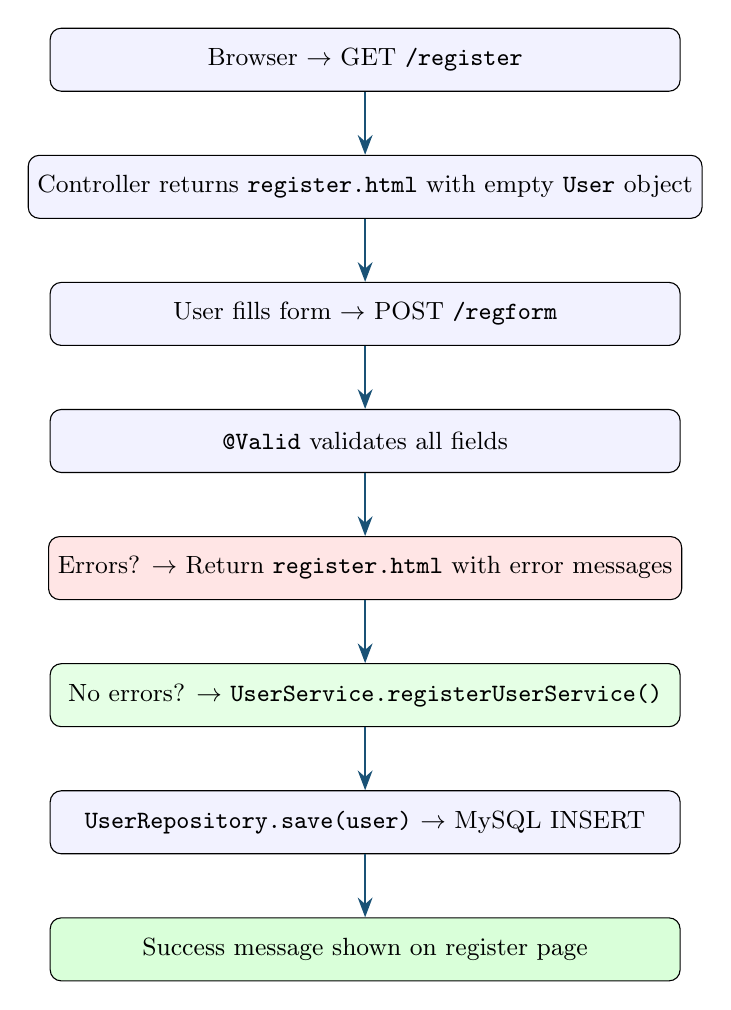
\begin{tikzpicture}[
    node distance=0.8cm,
    every node/.style={draw, rounded corners, minimum width=8cm, minimum height=0.8cm, align=center, font=\small, fill=blue!5},
    arrow/.style={-{Stealth[length=2.5mm]}, thick, color=primaryblue}
]
\node (s1) {Browser $\rightarrow$ GET \texttt{/register}};
\node (s2) [below=of s1] {Controller returns \texttt{register.html} with empty \texttt{User} object};
\node (s3) [below=of s2] {User fills form $\rightarrow$ POST \texttt{/regform}};
\node (s4) [below=of s3] {\texttt{@Valid} validates all fields};
\node (s5) [below=of s4, fill=red!10] {Errors? $\rightarrow$ Return \texttt{register.html} with error messages};
\node (s6) [below=of s5, fill=green!10] {No errors? $\rightarrow$ \texttt{UserService.registerUserService()}};
\node (s7) [below=of s6] {\texttt{UserRepository.save(user)} $\rightarrow$ MySQL INSERT};
\node (s8) [below=of s7, fill=green!15] {Success message shown on register page};

\draw[arrow] (s1) -- (s2);
\draw[arrow] (s2) -- (s3);
\draw[arrow] (s3) -- (s4);
\draw[arrow] (s4) -- (s5);
\draw[arrow] (s5) -- (s6);
\draw[arrow] (s6) -- (s7);
\draw[arrow] (s7) -- (s8);
\end{tikzpicture}
\end{center}

\subsection*{Purchase Flow}

\begin{center}
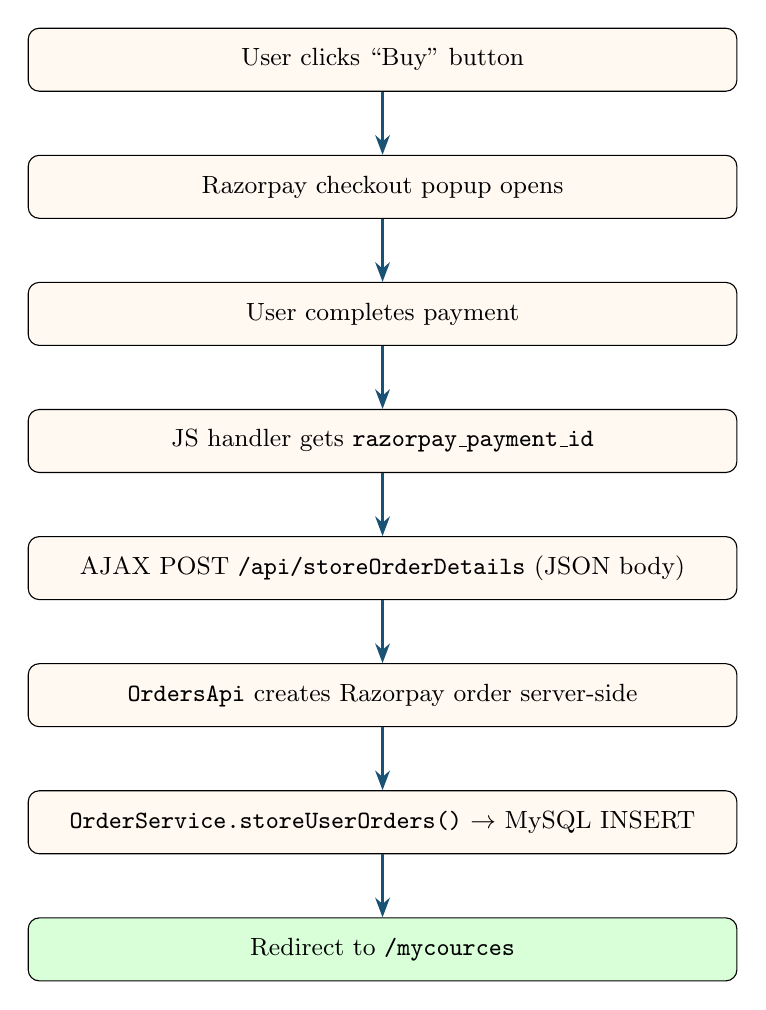
\begin{tikzpicture}[
    node distance=0.8cm,
    every node/.style={draw, rounded corners, minimum width=9cm, minimum height=0.8cm, align=center, font=\small, fill=orange!5},
    arrow/.style={-{Stealth[length=2.5mm]}, thick, color=primaryblue}
]
\node (p1) {User clicks ``Buy'' button};
\node (p2) [below=of p1] {Razorpay checkout popup opens};
\node (p3) [below=of p2] {User completes payment};
\node (p4) [below=of p3] {JS handler gets \texttt{razorpay\_payment\_id}};
\node (p5) [below=of p4] {AJAX POST \texttt{/api/storeOrderDetails} (JSON body)};
\node (p6) [below=of p5] {\texttt{OrdersApi} creates Razorpay order server-side};
\node (p7) [below=of p6] {\texttt{OrderService.storeUserOrders()} $\rightarrow$ MySQL INSERT};
\node (p8) [below=of p7, fill=green!15] {Redirect to \texttt{/mycources}};

\draw[arrow] (p1) -- (p2);
\draw[arrow] (p2) -- (p3);
\draw[arrow] (p3) -- (p4);
\draw[arrow] (p4) -- (p5);
\draw[arrow] (p5) -- (p6);
\draw[arrow] (p6) -- (p7);
\draw[arrow] (p7) -- (p8);
\end{tikzpicture}
\end{center}

% ======================================================================
\section{Database Questions}
% ======================================================================

\setcounter{subsection}{35}

% ---------- Q36 ----------
\subsection{Kaunsi database use ki aur kyun?}

\begin{answerbox}
\textbf{MySQL} --- relational database, structured data ke liye perfect (users, courses, orders). Free, widely used, Spring Boot ke saath excellent support via \texttt{mysql-connector-j}.
\end{answerbox}

% ---------- Q37 ----------
\subsection{Tables ka relationship kya hai?}

\begin{answerbox}
Currently \textbf{no foreign key relationship} defined in entities. Ideally:
\begin{itemize}
    \item Orders table ko User se \texttt{@ManyToOne} relationship honi chahiye
    \item Orders table ko Course se \texttt{@ManyToOne} relationship honi chahiye
    \item User ke \texttt{email} se Orders table mein \texttt{userEmail} match hota hai (loosely coupled)
\end{itemize}
\end{answerbox}

% ======================================================================
\section{Quick Revision Cheat Sheet}
% ======================================================================

\begin{center}
\begin{tcolorbox}[colback=answerbox, colframe=primaryblue, title={\large\bfseries Quick Revision Points}, fonttitle=\color{white}, coltitle=white, width=\textwidth]

\begin{tabular}{>{\bfseries}l p{10cm}}
Entities (3): & User, Course, Orders \\[3pt]
Repositories (3): & UserRepository, CourseRepository, OrdersRepository \\[3pt]
Services (3): & UserService, CourseService, OrderService \\[3pt]
Controller: & UserController (MVC) \\[3pt]
REST API: & OrdersApi \\[3pt]
Payment: & Razorpay (test mode, keys in code) \\[3pt]
Template Engine: & Thymeleaf with fragments \\[3pt]
Session: & \texttt{@SessionAttributes} for user login state \\[3pt]
Validation: & \texttt{@Pattern} regex + \texttt{@Valid} + \texttt{BindingResult} \\[3pt]
Database: & MySQL, JPA, Hibernate, \texttt{ddl-auto=update} \\[3pt]
Java Version: & 17 \\[3pt]
Spring Boot: & 4.0.2 \\[3pt]
\end{tabular}

\end{tcolorbox}
\end{center}

\newpage
% ======================================================================
% ======================================================================
%          PART 2 — JAVA INTERVIEW QUESTIONS (NON-COMMON)
% ======================================================================
% ======================================================================

\begin{center}
\begin{tcolorbox}[colback=warnbox, colframe=orange!80!black, width=\textwidth]
\centering
\Large\bfseries The following sections cover Java questions that \\
are \underline{definitely asked} in software development interviews \\
but most candidates skip or don't prepare well.
\end{tcolorbox}
\end{center}

% ======================================================================
\section{Core Java --- Beyond Basics}
% ======================================================================

\setcounter{subsection}{37}

% ---------- Q38 ----------
\subsection{String pool kya hai? \texttt{String s = "abc"} vs \texttt{new String("abc")} mein kya fark hai?}

\begin{answerbox}
\begin{itemize}
    \item \textbf{String Pool} (String Intern Pool) --- JVM ke Heap memory mein ek special area hai jahan unique string literals store hote hain.
    \item \texttt{String s1 = "abc";} $\rightarrow$ Pool mein check karega. Agar \texttt{"abc"} already hai toh same reference return karega. \textbf{No new object.}
    \item \texttt{String s2 = new String("abc");} $\rightarrow$ \textbf{Always new object} banata hai Heap mein (pool ke bahar). Plus agar \texttt{"abc"} pool mein nahi hai toh pool mein bhi ek object banayega.
\end{itemize}
\begin{lstlisting}[language=Java]
String s1 = "hello";
String s2 = "hello";
String s3 = new String("hello");

System.out.println(s1 == s2);      // true  (same pool reference)
System.out.println(s1 == s3);      // false (different objects)
System.out.println(s1.equals(s3)); // true  (same content)
\end{lstlisting}
\end{answerbox}

% ---------- Q39 ----------
\subsection{String immutable kyun hai? Iska kya fayda hai?}

\begin{answerbox}
\textbf{String immutable hai} matlab ek baar banne ke baad uska content change nahi ho sakta.\\[5pt]
\textbf{Reasons:}
\begin{enumerate}
    \item \textbf{String Pool possible hota hai} --- agar mutable hota toh ek reference change kare aur doosre ko bhi effect ho
    \item \textbf{Security} --- Database URL, passwords, file paths Strings mein hote hain. Immutable hone se koi tamper nahi kar sakta.
    \item \textbf{Thread Safety} --- Multiple threads safely share kar sakte hain bina synchronization ke
    \item \textbf{Hashcode Caching} --- HashMap mein key ke roop mein use hota hai, hashcode ek baar calculate hota hai aur cache hota hai
\end{enumerate}
\textbf{Mutable alternatives:} \texttt{StringBuilder} (not thread-safe, fast), \texttt{StringBuffer} (thread-safe, slow)
\end{answerbox}

% ---------- Q40 ----------
\subsection{\texttt{==} vs \texttt{.equals()} mein kya difference hai?}

\begin{answerbox}
\begin{center}
\begin{tabular}{p{6cm} p{6cm}}
\toprule
\textbf{\texttt{==}} & \textbf{\texttt{.equals()}} \\
\midrule
\textbf{Reference comparison} --- dono variables same object ko point karte hain ya nahi & \textbf{Content comparison} --- dono objects ka data/value same hai ya nahi \\
Primitives ke liye value compare karta hai & Only objects ke liye \\
Override nahi kar sakte & Override kar sakte hain (String, Integer ne kiya hai) \\
\bottomrule
\end{tabular}
\end{center}
\begin{lstlisting}[language=Java]
Integer a = 128;
Integer b = 128;
System.out.println(a == b);      // false (Integer cache -128 to 127)
System.out.println(a.equals(b)); // true

Integer c = 127;
Integer d = 127;
System.out.println(c == d);      // true (cached range)
\end{lstlisting}
\end{answerbox}

% ---------- Q41 ----------
\subsection{\texttt{final}, \texttt{finally}, \texttt{finalize} mein kya difference hai?}

\begin{answerbox}
\begin{center}
\begin{tabular}{>{\ttfamily}l p{9cm}}
\toprule
\textbf{Keyword} & \textbf{Purpose} \\
\midrule
final & \textbf{Variable:} constant (reassign nahi ho sakta) \newline \textbf{Method:} override nahi ho sakta \newline \textbf{Class:} inherit nahi ho sakti (e.g., \texttt{String}) \\
\midrule
finally & Try-catch ke saath \texttt{finally} block \textbf{hamesha execute hota hai} (cleanup code --- close connection, file) \\
\midrule
finalize() & Garbage Collector call karta hai object destroy karne se pehle. \textbf{Java 9+ mein deprecated hai.} \\
\bottomrule
\end{tabular}
\end{center}
\end{answerbox}

% ---------- Q42 ----------
\subsection{Checked vs Unchecked Exceptions mein kya fark hai?}

\begin{answerbox}
\begin{center}
\begin{tabular}{p{6cm} p{6cm}}
\toprule
\textbf{Checked Exception} & \textbf{Unchecked Exception} \\
\midrule
Compile-time pe check hota hai & Runtime pe aata hai \\
\texttt{try-catch} ya \texttt{throws} mandatory hai & Handle karna optional hai \\
\texttt{IOException}, \texttt{SQLException}, \texttt{FileNotFoundException} & \texttt{NullPointerException}, \texttt{ArrayIndexOutOfBoundsException}, \texttt{ArithmeticException} \\
\texttt{Exception} class extend karte hain & \texttt{RuntimeException} class extend karte hain \\
\bottomrule
\end{tabular}
\end{center}
\begin{lstlisting}[language=Java]
// Checked - must handle
try {
    FileReader fr = new FileReader("file.txt");
} catch (FileNotFoundException e) {
    e.printStackTrace();
}

// Unchecked - compiles without try-catch
int x = 10 / 0; // ArithmeticException at runtime
\end{lstlisting}
\end{answerbox}

% ---------- Q43 ----------
\subsection{\texttt{HashMap} internally kaise kaam karta hai?}

\begin{answerbox}
\textbf{Internal Working (bahut important question):}
\begin{enumerate}
    \item HashMap internally \textbf{Array of Nodes} (buckets) use karta hai. Default size = \textbf{16}.
    \item Jab \texttt{put(key, value)} call hota hai:
    \begin{enumerate}
        \item Key ka \texttt{hashCode()} calculate hota hai
        \item Hash se \textbf{bucket index} milta hai: \texttt{index = hash \& (n-1)}
        \item Agar bucket empty hai $\rightarrow$ direct store
        \item Agar collision hai (same index) $\rightarrow$ \textbf{LinkedList} banta hai (Java 8+ mein 8 nodes ke baad \textbf{Red-Black Tree} ban jaata hai)
    \end{enumerate}
    \item Jab \texttt{get(key)} call hota hai:
    \begin{enumerate}
        \item hashCode() se bucket find karo
        \item Bucket mein \texttt{equals()} se exact key match karo
        \item Value return karo
    \end{enumerate}
    \item \textbf{Load Factor = 0.75} --- jab 75\% buckets bhar jayein toh \textbf{rehashing} hota hai (size double: 16 $\rightarrow$ 32)
\end{enumerate}
\end{answerbox}

% ---------- Q44 ----------
\subsection{\texttt{HashMap} vs \texttt{HashTable} vs \texttt{ConcurrentHashMap} mein kya fark hai?}

\begin{answerbox}
\begin{center}
\begin{tabular}{p{3.5cm} p{3.5cm} p{4.5cm}}
\toprule
\textbf{HashMap} & \textbf{HashTable} & \textbf{ConcurrentHashMap} \\
\midrule
Not synchronized & Synchronized (whole map lock) & Segment-level locking \\
Allows 1 null key & No null key/value & No null key/value \\
Fast (single-thread) & Slow (full lock) & Fast (multi-thread) \\
Not thread-safe & Thread-safe & Thread-safe \\
Java 1.2 & Java 1.0 (legacy) & Java 1.5+ (preferred) \\
\bottomrule
\end{tabular}
\end{center}
\textbf{Interview mein bolo:} ``Production mein multi-threaded environment ke liye \texttt{ConcurrentHashMap} use karte hain, \texttt{HashTable} legacy hai.''
\end{answerbox}

% ---------- Q45 ----------
\subsection{\texttt{ArrayList} vs \texttt{LinkedList} kab use karein?}

\begin{answerbox}
\begin{center}
\begin{tabular}{p{6cm} p{6cm}}
\toprule
\textbf{ArrayList} & \textbf{LinkedList} \\
\midrule
Internal: \textbf{Dynamic Array} & Internal: \textbf{Doubly Linked List} \\
\texttt{get(index)} $\rightarrow$ O(1) fast & \texttt{get(index)} $\rightarrow$ O(n) slow \\
\texttt{add/remove} middle $\rightarrow$ O(n) slow & \texttt{add/remove} $\rightarrow$ O(1) fast \\
Less memory (only data) & More memory (data + 2 pointers) \\
Best for: \textbf{read-heavy} operations & Best for: \textbf{insert/delete-heavy} operations \\
\bottomrule
\end{tabular}
\end{center}
\textbf{Real-world:} 90\% cases mein \texttt{ArrayList} use hota hai kyunki read operations zyada common hain.
\end{answerbox}

% ---------- Q46 ----------
\subsection{\texttt{Comparable} vs \texttt{Comparator} mein kya fark hai?}

\begin{answerbox}
\begin{center}
\begin{tabular}{p{6cm} p{6cm}}
\toprule
\textbf{Comparable} & \textbf{Comparator} \\
\midrule
\texttt{java.lang} package & \texttt{java.util} package \\
\texttt{compareTo()} method & \texttt{compare()} method \\
Class ke andar implement karo & Alag class mein define karo \\
\textbf{Natural ordering} (ek tarika) & \textbf{Custom ordering} (multiple tarike) \\
\texttt{Collections.sort(list)} & \texttt{Collections.sort(list, comparator)} \\
\bottomrule
\end{tabular}
\end{center}
\begin{lstlisting}[language=Java]
// Comparable - inside class
class Student implements Comparable<Student> {
    public int compareTo(Student s) {
        return this.name.compareTo(s.name); // sort by name
    }
}

// Comparator - external, multiple sort options
Collections.sort(list, (a, b) -> a.getAge() - b.getAge());
\end{lstlisting}
\end{answerbox}

% ======================================================================
\section{Java 8+ Features (Bahut Important)}
% ======================================================================

\setcounter{subsection}{46}

% ---------- Q47 ----------
\subsection{Lambda Expression kya hai? Kab use karte hain?}

\begin{answerbox}
Lambda expression ek \textbf{anonymous function} hai --- bina naam ke function likho.\\[5pt]
\textbf{Syntax:} \texttt{(parameters) -> \{body\}}\\[5pt]
\textbf{Use:} Jab \textbf{Functional Interface} (single abstract method wala interface) implement karna ho.
\begin{lstlisting}[language=Java]
// Before Java 8
Runnable r = new Runnable() {
    public void run() {
        System.out.println("Hello");
    }
};

// After Java 8 - Lambda
Runnable r = () -> System.out.println("Hello");

// With parameters
Comparator<String> comp = (a, b) -> a.compareTo(b);

// In Collections
list.forEach(item -> System.out.println(item));
list.sort((a, b) -> a.getName().compareTo(b.getName()));
\end{lstlisting}
\end{answerbox}

% ---------- Q48 ----------
\subsection{Functional Interface kya hai? Examples do.}

\begin{answerbox}
Woh interface jisme \textbf{exactly 1 abstract method} ho. \texttt{@FunctionalInterface} annotation optional hai but recommended.
\begin{center}
\begin{tabular}{>{\ttfamily}l l l}
\toprule
\textbf{Interface} & \textbf{Method} & \textbf{Use Case} \\
\midrule
Predicate<T> & test(T) $\rightarrow$ boolean & Filtering \\
Function<T,R> & apply(T) $\rightarrow$ R & Transformation \\
Consumer<T> & accept(T) $\rightarrow$ void & forEach actions \\
Supplier<T> & get() $\rightarrow$ T & Object creation \\
Runnable & run() $\rightarrow$ void & Thread execution \\
Comparator<T> & compare(T,T) $\rightarrow$ int & Sorting \\
\bottomrule
\end{tabular}
\end{center}
\begin{lstlisting}[language=Java]
Predicate<Integer> isEven = n -> n % 2 == 0;
System.out.println(isEven.test(4)); // true

Function<String, Integer> length = s -> s.length();
System.out.println(length.apply("hello")); // 5
\end{lstlisting}
\end{answerbox}

% ---------- Q49 ----------
\subsection{Stream API kya hai? Example ke saath samjhao.}

\begin{answerbox}
Stream API collections ke upar \textbf{functional-style operations} karne deta hai --- filter, map, reduce, collect etc.\\[5pt]
\textbf{Key points:}
\begin{itemize}
    \item Stream data ko \textbf{modify nahi karta} (original collection safe)
    \item \textbf{Lazy evaluation} --- terminal operation ke bina intermediate operations execute nahi hote
    \item \textbf{One-time use} --- ek stream dobara use nahi ho sakta
\end{itemize}
\begin{lstlisting}[language=Java]
List<String> names = Arrays.asList("Gaurav","Amit","Rahul","Ankit","Ravi");

// Filter names starting with 'A', convert to uppercase, collect
List<String> result = names.stream()
    .filter(n -> n.startsWith("A"))      // Intermediate
    .map(String::toUpperCase)            // Intermediate
    .sorted()                            // Intermediate
    .collect(Collectors.toList());       // Terminal
// Output: [AMIT, ANKIT]

// Count, Sum, Average
long count = names.stream().filter(n -> n.length() > 4).count();

// Find first
Optional<String> first = names.stream()
    .filter(n -> n.startsWith("R"))
    .findFirst();
\end{lstlisting}
\end{answerbox}

% ---------- Q50 ----------
\subsection{\texttt{Optional} class kya hai? \texttt{NullPointerException} kaise avoid karta hai?}

\begin{answerbox}
\texttt{Optional<T>} ek container hai jo \textbf{value hold kar sakta hai ya empty ho sakta hai}. NullPointerException avoid karne ke liye Java 8 mein introduce hua.
\begin{lstlisting}[language=Java]
// Without Optional - NullPointerException risk
User user = userRepository.findByEmail("abc@gmail.com");
String name = user.getName(); // BOOM if user is null!

// With Optional - Safe
Optional<User> optUser = Optional.ofNullable(user);
String name = optUser
    .map(User::getName)
    .orElse("Unknown");          // default value if empty

// Other useful methods
optUser.isPresent();             // true/false
optUser.ifPresent(u -> log(u));  // execute if value exists
optUser.orElseThrow(() -> new RuntimeException("Not found"));
\end{lstlisting}
\end{answerbox}

% ---------- Q51 ----------
\subsection{\texttt{map()} vs \texttt{flatMap()} mein kya fark hai?}

\begin{answerbox}
\begin{center}
\begin{tabular}{p{6cm} p{6cm}}
\toprule
\textbf{\texttt{map()}} & \textbf{\texttt{flatMap()}} \\
\midrule
1-to-1 transformation & 1-to-many + flatten \\
Returns: \texttt{Stream<Stream<T>>} agar inner stream ho & Returns: \texttt{Stream<T>} (flattened) \\
Simple mapping & Nested collections flatten karna \\
\bottomrule
\end{tabular}
\end{center}
\begin{lstlisting}[language=Java]
// map - each element transforms to one element
List<String> names = List.of("Gaurav", "Amit");
List<Integer> lengths = names.stream()
    .map(String::length)
    .collect(Collectors.toList()); // [6, 4]

// flatMap - each element transforms to multiple, then flatten
List<List<Integer>> nested = List.of(
    List.of(1,2,3), List.of(4,5,6));
List<Integer> flat = nested.stream()
    .flatMap(Collection::stream)
    .collect(Collectors.toList()); // [1,2,3,4,5,6]
\end{lstlisting}
\end{answerbox}

% ---------- Q52 ----------
\subsection{Method Reference kya hai? Types batao.}

\begin{answerbox}
Method reference lambda ka shortcut hai jab lambda sirf ek method call karta hai.\\[5pt]
\textbf{Syntax:} \texttt{ClassName::methodName}
\begin{center}
\begin{tabular}{l l l}
\toprule
\textbf{Type} & \textbf{Syntax} & \textbf{Lambda Equivalent} \\
\midrule
Static method & \texttt{Math::max} & \texttt{(a,b) -> Math.max(a,b)} \\
Instance method & \texttt{str::toUpperCase} & \texttt{() -> str.toUpperCase()} \\
Arbitrary object & \texttt{String::length} & \texttt{s -> s.length()} \\
Constructor & \texttt{ArrayList::new} & \texttt{() -> new ArrayList()} \\
\bottomrule
\end{tabular}
\end{center}
\begin{lstlisting}[language=Java]
list.forEach(System.out::println);  // Method reference
list.forEach(s -> System.out.println(s)); // Equivalent lambda
\end{lstlisting}
\end{answerbox}

% ======================================================================
\section{Multithreading \& Concurrency}
% ======================================================================

\setcounter{subsection}{52}

% ---------- Q53 ----------
\subsection{Thread create karne ke kitne tarike hain?}

\begin{answerbox}
\textbf{4 tarike:}
\begin{lstlisting}[language=Java]
// 1. Extend Thread class
class MyThread extends Thread {
    public void run() { System.out.println("Thread 1"); }
}
new MyThread().start();

// 2. Implement Runnable interface (PREFERRED)
class MyRunnable implements Runnable {
    public void run() { System.out.println("Thread 2"); }
}
new Thread(new MyRunnable()).start();

// 3. Lambda (Java 8+)
new Thread(() -> System.out.println("Thread 3")).start();

// 4. Callable + Future (returns value)
Callable<String> task = () -> "Result";
ExecutorService executor = Executors.newSingleThreadExecutor();
Future<String> future = executor.submit(task);
String result = future.get(); // blocks until done
\end{lstlisting}
\textbf{Why Runnable preferred over Thread?}
\begin{itemize}
    \item Java supports single inheritance --- Thread extend karoge toh doosri class extend nahi kar sakte
    \item Runnable implement karke multiple interface implement ho sakte hain
    \item Separation of concerns --- task alag, execution alag
\end{itemize}
\end{answerbox}

% ---------- Q54 ----------
\subsection{\texttt{synchronized} keyword kya karta hai?}

\begin{answerbox}
\begin{itemize}
    \item Ek time pe \textbf{sirf ek thread} us block/method ko access kar sake --- \textbf{mutual exclusion}
    \item \textbf{Thread-safety} provide karta hai shared data ke liye
    \item Ek thread lock acquire karta hai, doosre wait karte hain
\end{itemize}
\begin{lstlisting}[language=Java]
// Synchronized method
public synchronized void increment() {
    count++;
}

// Synchronized block (more granular)
public void increment() {
    synchronized(this) {
        count++;
    }
}
\end{lstlisting}
\textbf{Problem:} Performance slow hoti hai kyunki threads wait karte hain.\\
\textbf{Alternative:} \texttt{volatile}, \texttt{AtomicInteger}, \texttt{ReentrantLock}, \texttt{ConcurrentHashMap}
\end{answerbox}

% ---------- Q55 ----------
\subsection{Thread lifecycle (states) kya hain?}

\begin{answerbox}
\begin{center}
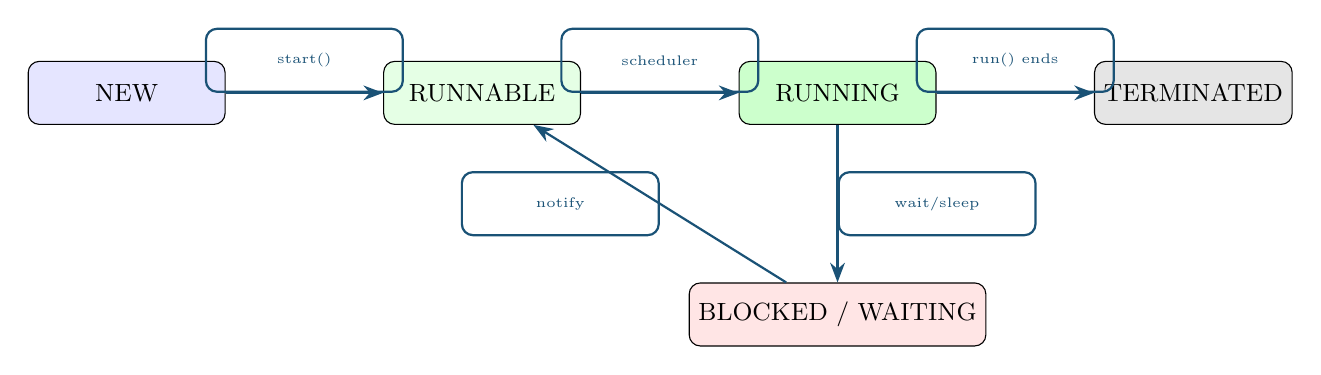
\begin{tikzpicture}[
    node distance=2cm,
    every node/.style={draw, rounded corners, minimum width=2.5cm, minimum height=0.8cm, align=center, font=\small},
    arrow/.style={-{Stealth[length=2.5mm]}, thick, color=primaryblue}
]
\node (new) [fill=blue!10] {NEW};
\node (run) [right=of new, fill=green!10] {RUNNABLE};
\node (running) [right=of run, fill=green!20] {RUNNING};
\node (blocked) [below=of running, fill=red!10] {BLOCKED / WAITING};
\node (dead) [right=of running, fill=gray!20] {TERMINATED};

\draw[arrow] (new) -- node[above, font=\tiny] {start()} (run);
\draw[arrow] (run) -- node[above, font=\tiny] {scheduler} (running);
\draw[arrow] (running) -- node[above, font=\tiny] {run() ends} (dead);
\draw[arrow] (running) -- node[right, font=\tiny] {wait/sleep} (blocked);
\draw[arrow] (blocked) -- node[left, font=\tiny] {notify} (run);
\end{tikzpicture}
\end{center}
\begin{enumerate}
    \item \textbf{NEW} --- Thread object created, \texttt{start()} not called yet
    \item \textbf{RUNNABLE} --- \texttt{start()} called, ready to run, waiting for CPU
    \item \textbf{RUNNING} --- Thread is executing \texttt{run()} method
    \item \textbf{BLOCKED/WAITING} --- \texttt{wait()}, \texttt{sleep()}, waiting for lock
    \item \textbf{TERMINATED} --- \texttt{run()} method completed
\end{enumerate}
\end{answerbox}

% ---------- Q56 ----------
\subsection{\texttt{wait()} vs \texttt{sleep()} mein kya fark hai?}

\begin{answerbox}
\begin{center}
\begin{tabular}{p{6cm} p{6cm}}
\toprule
\textbf{\texttt{wait()}} & \textbf{\texttt{sleep()}} \\
\midrule
\texttt{Object} class ka method & \texttt{Thread} class ka method \\
\textbf{Lock release} karta hai & \textbf{Lock release nahi} karta \\
\texttt{notify()} / \texttt{notifyAll()} se wake up & Time complete hone pe auto wake up \\
\texttt{synchronized} block mein use hota hai & Kahin bhi use ho sakta \\
Inter-thread communication ke liye & Pause/delay ke liye \\
\bottomrule
\end{tabular}
\end{center}
\end{answerbox}

% ======================================================================
\section{OOP Concepts --- Deep Dive}
% ======================================================================

\setcounter{subsection}{56}

% ---------- Q57 ----------
\subsection{Abstract class vs Interface mein kya fark hai? (Java 8+ ke baad)}

\begin{answerbox}
\begin{center}
\begin{tabular}{p{6cm} p{6cm}}
\toprule
\textbf{Abstract Class} & \textbf{Interface} \\
\midrule
\texttt{abstract} keyword & \texttt{interface} keyword \\
Abstract + concrete methods & Abstract + \texttt{default} + \texttt{static} methods (Java 8+) \\
Instance variables ho sakte hain & Only \texttt{public static final} constants \\
Constructor ho sakta hai & Constructor nahi ho sakta \\
\texttt{extends} (single) & \texttt{implements} (multiple) \\
Any access modifier & Methods \texttt{public} by default \\
\bottomrule
\end{tabular}
\end{center}

\textbf{Kab use karein:}
\begin{itemize}
    \item \textbf{Abstract class} $\rightarrow$ jab classes ke beech \textbf{IS-A relationship} ho aur common code share karna ho
    \item \textbf{Interface} $\rightarrow$ jab unrelated classes ko \textbf{same capability} deni ho (e.g., \texttt{Serializable}, \texttt{Comparable})
\end{itemize}
\end{answerbox}

% ---------- Q58 ----------
\subsection{Method Overloading vs Overriding mein kya fark hai?}

\begin{answerbox}
\begin{center}
\begin{tabular}{p{6cm} p{6cm}}
\toprule
\textbf{Overloading} & \textbf{Overriding} \\
\midrule
\textbf{Same class} mein & \textbf{Parent-child} class mein \\
Same method name, \textbf{different parameters} & Same method name, \textbf{same parameters} \\
\textbf{Compile-time} polymorphism & \textbf{Runtime} polymorphism \\
Return type different ho sakta hai & Return type same ya covariant \\
\texttt{static} methods overload ho sakte hain & \texttt{static} methods override nahi hote \\
\bottomrule
\end{tabular}
\end{center}
\begin{lstlisting}[language=Java]
// Overloading
class Calculator {
    int add(int a, int b) { return a + b; }
    double add(double a, double b) { return a + b; }
}

// Overriding
class Animal { void sound() { System.out.println("..."); } }
class Dog extends Animal {
    @Override
    void sound() { System.out.println("Bark"); }
}
\end{lstlisting}
\end{answerbox}

% ---------- Q59 ----------
\subsection{Singleton Design Pattern kaise implement karein?}

\begin{answerbox}
Singleton pattern ensures \textbf{class ka sirf ek object} bane poore application mein (e.g., Database connection, Logger).
\begin{lstlisting}[language=Java]
// Thread-Safe Singleton (Best approach)
public class DatabaseConnection {
    private static volatile DatabaseConnection instance;
    
    private DatabaseConnection() { } // private constructor
    
    public static DatabaseConnection getInstance() {
        if (instance == null) {                    // 1st check
            synchronized (DatabaseConnection.class) {
                if (instance == null) {            // 2nd check
                    instance = new DatabaseConnection();
                }
            }
        }
        return instance;
    }
}

// Usage
DatabaseConnection db = DatabaseConnection.getInstance();
\end{lstlisting}
\textbf{Spring mein:} Beans by default \textbf{Singleton scope} mein hote hain --- Spring container ek hi instance banata hai.
\end{answerbox}

% ---------- Q60 ----------
\subsection{Immutable class kaise banate hain?}

\begin{answerbox}
\begin{enumerate}
    \item Class ko \texttt{final} declare karo (inheritance prevent)
    \item Sab fields \texttt{private final} karo
    \item Constructor se initialize karo
    \item Sirf \textbf{getters} do, \textbf{no setters}
    \item Mutable objects ka \textbf{deep copy} return karo getter mein
\end{enumerate}
\begin{lstlisting}[language=Java]
public final class Student {
    private final String name;
    private final int age;
    
    public Student(String name, int age) {
        this.name = name;
        this.age = age;
    }
    
    public String getName() { return name; }
    public int getAge() { return age; }
    // No setters!
}
\end{lstlisting}
\textbf{Examples:} \texttt{String}, \texttt{Integer}, \texttt{LocalDate} --- sab immutable hain.
\end{answerbox}

% ======================================================================
\section{Spring Boot --- Deep Dive Questions}
% ======================================================================

\setcounter{subsection}{60}

% ---------- Q61 ----------
\subsection{Spring Bean Lifecycle kya hai?}

\begin{answerbox}
\begin{enumerate}
    \item \textbf{Instantiation} --- Spring container bean object create karta hai
    \item \textbf{Populate Properties} --- Dependencies inject hoti hain (\texttt{@Autowired})
    \item \textbf{BeanNameAware} --- Bean ko apna naam pata chalta hai
    \item \textbf{BeanFactoryAware} --- Bean ko factory ka reference milta hai
    \item \textbf{Pre-initialization} --- \texttt{@PostConstruct} method call hota hai
    \item \textbf{InitializingBean} --- \texttt{afterPropertiesSet()} call hota hai
    \item \textbf{Custom init method} --- \texttt{@Bean(initMethod="init")}
    \item \textbf{Bean is READY to use}
    \item \textbf{Pre-destroy} --- \texttt{@PreDestroy} method call hota hai
    \item \textbf{DisposableBean} --- \texttt{destroy()} call hota hai
\end{enumerate}
\textbf{Most commonly used:} \texttt{@PostConstruct} (init) aur \texttt{@PreDestroy} (cleanup)
\end{answerbox}

% ---------- Q62 ----------
\subsection{Spring Bean Scopes kaunse hain?}

\begin{answerbox}
\begin{center}
\begin{tabular}{>{\ttfamily}l p{8cm}}
\toprule
\textbf{Scope} & \textbf{Description} \\
\midrule
singleton & \textbf{Default.} Ek hi instance poore application mein. \\
prototype & Har request pe naya instance banta hai. \\
request & Har HTTP request ke liye ek instance (Web app only). \\
session & Har HTTP session ke liye ek instance. \\
application & Har ServletContext ke liye ek instance. \\
\bottomrule
\end{tabular}
\end{center}
\begin{lstlisting}[language=Java]
@Service
@Scope("prototype") // new instance every time
public class ReportService { }
\end{lstlisting}
\end{answerbox}

% ---------- Q63 ----------
\subsection{\texttt{@ControllerAdvice} se Global Exception Handling kaise karein?}

\begin{answerbox}
\texttt{@ControllerAdvice} ek \textbf{centralized exception handler} hai --- sab controllers ke exceptions ek jagah handle hote hain.
\begin{lstlisting}[language=Java]
@ControllerAdvice
public class GlobalExceptionHandler {

    @ExceptionHandler(NullPointerException.class)
    public ResponseEntity<String> handleNull(NullPointerException e) {
        return ResponseEntity.status(500)
            .body("Something went wrong: " + e.getMessage());
    }
    
    @ExceptionHandler(Exception.class)
    public ResponseEntity<String> handleAll(Exception e) {
        return ResponseEntity.status(500)
            .body("Internal Server Error");
    }
}
\end{lstlisting}
\textbf{Why use?}
\begin{itemize}
    \item Har controller mein try-catch likhne ki zaroorat nahi
    \item Clean, maintainable error handling
    \item Consistent error responses
\end{itemize}
\end{answerbox}

% ---------- Q64 ----------
\subsection{Spring Boot mein \texttt{@Transactional} kya karta hai?}

\begin{answerbox}
\begin{itemize}
    \item Method ke andar sab database operations \textbf{ek transaction} mein wrap ho jaate hain
    \item Agar koi exception aaye $\rightarrow$ \textbf{ROLLBACK} (sab changes undo)
    \item Sab successful $\rightarrow$ \textbf{COMMIT}
\end{itemize}
\begin{lstlisting}[language=Java]
@Service
public class OrderService {
    @Transactional
    public void placeOrder(Order order) {
        orderRepo.save(order);          // Step 1
        paymentRepo.deduct(amount);     // Step 2
        inventoryRepo.reduce(item);     // Step 3
        // If Step 3 fails -> Step 1 & 2 ROLLBACK
    }
}
\end{lstlisting}
\textbf{ACID Properties:}
\begin{itemize}
    \item \textbf{A}tomicity --- all or nothing
    \item \textbf{C}onsistency --- valid state to valid state
    \item \textbf{I}solation --- concurrent transactions don't interfere
    \item \textbf{D}urability --- committed data persists
\end{itemize}
\end{answerbox}

% ---------- Q65 ----------
\subsection{Spring Boot Actuator kya hai?}

\begin{answerbox}
\begin{itemize}
    \item Production-ready features provide karta hai --- \textbf{health check, metrics, monitoring}
    \item Dependency: \texttt{spring-boot-starter-actuator}
    \item Endpoints:
    \begin{itemize}
        \item \texttt{/actuator/health} --- application up/down status
        \item \texttt{/actuator/info} --- application info
        \item \texttt{/actuator/metrics} --- JVM memory, CPU, thread count
        \item \texttt{/actuator/env} --- environment properties
    \end{itemize}
\end{itemize}
\end{answerbox}

% ---------- Q66 ----------
\subsection{Dependency Injection ke types kaunse hain? Best practice kya hai?}

\begin{answerbox}
\begin{lstlisting}[language=Java]
// 1. Field Injection (NOT recommended)
@Autowired
private UserService userService;

// 2. Setter Injection
@Autowired
public void setUserService(UserService userService) {
    this.userService = userService;
}

// 3. Constructor Injection (BEST PRACTICE)
private final UserService userService;

@Autowired // optional if single constructor
public UserController(UserService userService) {
    this.userService = userService;
}
\end{lstlisting}
\textbf{Why Constructor Injection is best:}
\begin{enumerate}
    \item Fields \texttt{final} ho sakte hain $\rightarrow$ \textbf{immutable}
    \item Mandatory dependencies clearly visible
    \item Unit testing easy (constructor se mock inject karo)
    \item No reflection needed (unlike field injection)
\end{enumerate}
\end{answerbox}

% ======================================================================
\section{Hibernate / JPA --- Deep Dive}
% ======================================================================

\setcounter{subsection}{66}

% ---------- Q67 ----------
\subsection{Hibernate mein \texttt{get()} vs \texttt{load()} mein kya fark hai?}

\begin{answerbox}
\begin{center}
\begin{tabular}{p{6cm} p{6cm}}
\toprule
\textbf{\texttt{get()}} & \textbf{\texttt{load()}} \\
\midrule
Database hit \textbf{turant} hota hai & \textbf{Lazy loading} --- proxy return karta hai, DB hit tab hota hai jab property access ho \\
Object nahi mila $\rightarrow$ \texttt{null} return & Object nahi mila $\rightarrow$ \texttt{ObjectNotFoundException} \\
Jab sure nahi ho ki exist karta hai & Jab sure ho ki exist karta hai \\
\bottomrule
\end{tabular}
\end{center}
\end{answerbox}

% ---------- Q68 ----------
\subsection{Lazy Loading vs Eager Loading kya hai?}

\begin{answerbox}
\begin{center}
\begin{tabular}{p{6cm} p{6cm}}
\toprule
\textbf{Lazy Loading} & \textbf{Eager Loading} \\
\midrule
Related data \textbf{tab load} hota hai jab access karo & Related data \textbf{saath mein} load hota hai (JOIN query) \\
\texttt{FetchType.LAZY} (default for collections) & \texttt{FetchType.EAGER} (default for single) \\
Better performance (on-demand) & N+1 query problem avoid karta hai \\
\bottomrule
\end{tabular}
\end{center}
\begin{lstlisting}[language=Java]
@OneToMany(fetch = FetchType.LAZY)  // courses tab load jab access
private List<Course> courses;

@ManyToOne(fetch = FetchType.EAGER) // user saath mein load
private User user;
\end{lstlisting}
\textbf{N+1 Problem:} 10 orders fetch kiye, har order ke user ke liye alag query $=$ 1 + 10 $=$ 11 queries! Solution: \texttt{JOIN FETCH} ya \texttt{@EntityGraph}
\end{answerbox}

% ---------- Q69 ----------
\subsection{JPA entity states kaunse hain? (Entity Lifecycle)}

\begin{answerbox}
\begin{enumerate}
    \item \textbf{Transient} --- \texttt{new User()} --- object banaya but DB se koi connection nahi
    \item \textbf{Persistent/Managed} --- \texttt{entityManager.persist(user)} ya \texttt{repo.save()} --- Hibernate track kar raha hai, changes automatically sync
    \item \textbf{Detached} --- Session close hone ke baad --- object hai but Hibernate track nahi kar raha
    \item \textbf{Removed} --- \texttt{entityManager.remove(user)} --- delete ke liye mark hua
\end{enumerate}
\begin{lstlisting}[language=Java]
User user = new User();          // TRANSIENT
entityManager.persist(user);      // PERSISTENT
entityManager.detach(user);       // DETACHED
entityManager.merge(user);        // PERSISTENT again
entityManager.remove(user);       // REMOVED
\end{lstlisting}
\end{answerbox}

% ---------- Q70 ----------
\subsection{JPA relationships explain karo with annotations.}

\begin{answerbox}
\begin{center}
\begin{tabular}{>{\ttfamily}l p{5cm} p{4cm}}
\toprule
\textbf{Annotation} & \textbf{Meaning} & \textbf{Example} \\
\midrule
@OneToOne & Ek entity $\leftrightarrow$ ek entity & User $\leftrightarrow$ Profile \\
@OneToMany & Ek entity $\leftrightarrow$ many entities & User $\rightarrow$ Orders \\
@ManyToOne & Many entities $\rightarrow$ ek entity & Orders $\rightarrow$ User \\
@ManyToMany & Many $\leftrightarrow$ many & Student $\leftrightarrow$ Courses \\
\bottomrule
\end{tabular}
\end{center}
\begin{lstlisting}[language=Java]
@Entity
public class User {
    @OneToMany(mappedBy = "user", cascade = CascadeType.ALL)
    private List<Orders> orders;
}

@Entity
public class Orders {
    @ManyToOne
    @JoinColumn(name = "user_id")
    private User user;
}
\end{lstlisting}
\textbf{CascadeType.ALL} --- User save/delete hone pe uske sab orders bhi save/delete ho jayenge.
\end{answerbox}

% ======================================================================
\section{REST API Questions}
% ======================================================================

\setcounter{subsection}{70}

% ---------- Q71 ----------
\subsection{REST API kya hai? HTTP methods explain karo.}

\begin{answerbox}
\textbf{REST} (Representational State Transfer) --- ek architectural style hai stateless client-server communication ke liye.
\begin{center}
\begin{tabular}{>{\ttfamily}l l l}
\toprule
\textbf{Method} & \textbf{CRUD} & \textbf{Example} \\
\midrule
GET & Read & \texttt{GET /api/courses} \\
POST & Create & \texttt{POST /api/courses} \\
PUT & Update (full) & \texttt{PUT /api/courses/1} \\
PATCH & Update (partial) & \texttt{PATCH /api/courses/1} \\
DELETE & Delete & \texttt{DELETE /api/courses/1} \\
\bottomrule
\end{tabular}
\end{center}
\textbf{REST principles:}
\begin{enumerate}
    \item \textbf{Stateless} --- server koi client state store nahi karta
    \item \textbf{Uniform Interface} --- standard HTTP methods use karo
    \item \textbf{Resource-based} --- URL resources represent karte hain (\texttt{/users}, \texttt{/courses})
    \item \textbf{JSON} --- data exchange format
\end{enumerate}
\end{answerbox}

% ---------- Q72 ----------
\subsection{HTTP Status Codes kaunse important hain?}

\begin{answerbox}
\begin{center}
\begin{tabular}{l l l}
\toprule
\textbf{Code} & \textbf{Meaning} & \textbf{When} \\
\midrule
200 & OK & Successful GET/PUT \\
201 & Created & Successful POST (new resource) \\
204 & No Content & Successful DELETE \\
400 & Bad Request & Invalid input / validation fail \\
401 & Unauthorized & Not logged in \\
403 & Forbidden & Logged in but no permission \\
404 & Not Found & Resource doesn't exist \\
405 & Method Not Allowed & Wrong HTTP method \\
500 & Internal Server Error & Server-side exception \\
\bottomrule
\end{tabular}
\end{center}
\end{answerbox}

% ---------- Q73 ----------
\subsection{\texttt{@PathVariable} vs \texttt{@RequestParam} mein kya fark hai?}

\begin{answerbox}
\begin{lstlisting}[language=Java]
// @PathVariable - URL path ka part
// URL: /api/users/5
@GetMapping("/api/users/{id}")
public User getUser(@PathVariable Long id) { }

// @RequestParam - Query parameter (? ke baad)
// URL: /api/users?city=Delhi&page=1
@GetMapping("/api/users")
public List<User> getUsers(
    @RequestParam String city,
    @RequestParam(defaultValue = "1") int page) { }
\end{lstlisting}
\begin{center}
\begin{tabular}{p{6cm} p{6cm}}
\toprule
\textbf{\texttt{@PathVariable}} & \textbf{\texttt{@RequestParam}} \\
\midrule
URL path mein: \texttt{/users/\{id\}} & Query string mein: \texttt{/users?id=5} \\
Mandatory by default & Optional with default value \\
Specific resource identify karne ke liye & Filtering/pagination ke liye \\
\bottomrule
\end{tabular}
\end{center}
\end{answerbox}

% ======================================================================
\section{SQL Queries (Commonly Asked in Interviews)}
% ======================================================================

\setcounter{subsection}{73}

% ---------- Q74 ----------
\subsection{2nd highest salary kaise nikalenge?}

\begin{answerbox}
\begin{lstlisting}[language=SQL]
-- Method 1: Subquery
SELECT MAX(salary) FROM employee
WHERE salary < (SELECT MAX(salary) FROM employee);

-- Method 2: LIMIT + OFFSET
SELECT DISTINCT salary FROM employee
ORDER BY salary DESC LIMIT 1 OFFSET 1;

-- Method 3: Nth highest (generic)
SELECT salary FROM employee e1
WHERE N-1 = (SELECT COUNT(DISTINCT salary) FROM employee e2
             WHERE e2.salary > e1.salary);
\end{lstlisting}
\end{answerbox}

% ---------- Q75 ----------
\subsection{JOIN types explain karo.}

\begin{answerbox}
\begin{center}
\begin{tabular}{l p{8cm}}
\toprule
\textbf{JOIN} & \textbf{Result} \\
\midrule
\textbf{INNER JOIN} & Sirf matching rows dono tables se \\
\textbf{LEFT JOIN} & Left table ki sab rows + matching right rows (no match $\rightarrow$ NULL) \\
\textbf{RIGHT JOIN} & Right table ki sab rows + matching left rows \\
\textbf{FULL OUTER JOIN} & Dono tables ki sab rows (MySQL mein directly nahi, UNION se karo) \\
\textbf{CROSS JOIN} & Cartesian product --- har row doosri har row ke saath \\
\textbf{SELF JOIN} & Table apne aap se join --- e.g., employee-manager same table \\
\bottomrule
\end{tabular}
\end{center}
\begin{lstlisting}[language=SQL]
-- Find users who purchased courses
SELECT u.name, o.courseName 
FROM user u 
INNER JOIN orders o ON u.email = o.userEmail;

-- Find users with or without orders
SELECT u.name, o.courseName 
FROM user u 
LEFT JOIN orders o ON u.email = o.userEmail;
\end{lstlisting}
\end{answerbox}

% ---------- Q76 ----------
\subsection{GROUP BY, HAVING, aur aggregate functions}

\begin{answerbox}
\begin{lstlisting}[language=SQL]
-- Count orders per user
SELECT userEmail, COUNT(*) as total_orders 
FROM orders 
GROUP BY userEmail;

-- Users with more than 2 orders (HAVING filters groups)
SELECT userEmail, COUNT(*) as total_orders 
FROM orders 
GROUP BY userEmail 
HAVING COUNT(*) > 2;

-- Total revenue per course
SELECT courseName, SUM(CAST(courseAmount AS DECIMAL)) as revenue 
FROM orders 
GROUP BY courseName 
ORDER BY revenue DESC;
\end{lstlisting}
\textbf{WHERE vs HAVING:}
\begin{itemize}
    \item \texttt{WHERE} --- rows filter karta hai \textbf{GROUP BY se pehle}
    \item \texttt{HAVING} --- groups filter karta hai \textbf{GROUP BY ke baad}
\end{itemize}
\end{answerbox}

% ======================================================================
\section{Coding Problems (Interviewer Zaroor Puchega)}
% ======================================================================

\setcounter{subsection}{76}

% ---------- Q77 ----------
\subsection{String reverse karo (without \texttt{reverse()} method)}

\begin{answerbox}
\begin{lstlisting}[language=Java]
// Method 1: Loop
public String reverse(String str) {
    char[] arr = str.toCharArray();
    int left = 0, right = arr.length - 1;
    while (left < right) {
        char temp = arr[left];
        arr[left] = arr[right];
        arr[right] = temp;
        left++;
        right--;
    }
    return new String(arr);
}

// Method 2: StringBuilder
public String reverse(String str) {
    return new StringBuilder(str).reverse().toString();
}
\end{lstlisting}
\end{answerbox}

% ---------- Q78 ----------
\subsection{Check if String is Palindrome}

\begin{answerbox}
\begin{lstlisting}[language=Java]
public boolean isPalindrome(String str) {
    str = str.toLowerCase().replaceAll("[^a-z0-9]", "");
    int left = 0, right = str.length() - 1;
    while (left < right) {
        if (str.charAt(left) != str.charAt(right)) return false;
        left++;
        right--;
    }
    return true;
}
// "madam" -> true, "hello" -> false
\end{lstlisting}
\end{answerbox}

% ---------- Q79 ----------
\subsection{Find duplicate characters in a String}

\begin{answerbox}
\begin{lstlisting}[language=Java]
public void findDuplicates(String str) {
    Map<Character, Integer> map = new HashMap<>();
    for (char c : str.toCharArray()) {
        map.put(c, map.getOrDefault(c, 0) + 1);
    }
    map.entrySet().stream()
       .filter(e -> e.getValue() > 1)
       .forEach(e -> System.out.println(e.getKey() 
                     + " = " + e.getValue()));
}
// "programming" -> r=2, g=2, m=2
\end{lstlisting}
\end{answerbox}

% ---------- Q80 ----------
\subsection{Check if two Strings are Anagram}

\begin{answerbox}
\begin{lstlisting}[language=Java]
public boolean isAnagram(String s1, String s2) {
    if (s1.length() != s2.length()) return false;
    char[] a1 = s1.toLowerCase().toCharArray();
    char[] a2 = s2.toLowerCase().toCharArray();
    Arrays.sort(a1);
    Arrays.sort(a2);
    return Arrays.equals(a1, a2);
}
// "listen", "silent" -> true
\end{lstlisting}
\end{answerbox}

% ---------- Q81 ----------
\subsection{Fibonacci series print karo}

\begin{answerbox}
\begin{lstlisting}[language=Java]
// Iterative (Best)
public void fibonacci(int n) {
    int a = 0, b = 1;
    for (int i = 0; i < n; i++) {
        System.out.print(a + " ");
        int temp = a + b;
        a = b;
        b = temp;
    }
}
// fibonacci(7) -> 0 1 1 2 3 5 8

// Using Streams (Java 8+)
Stream.iterate(new int[]{0, 1}, f -> new int[]{f[1], f[0]+f[1]})
      .limit(7)
      .map(f -> f[0])
      .forEach(n -> System.out.print(n + " "));
\end{lstlisting}
\end{answerbox}

% ---------- Q82 ----------
\subsection{Array se duplicate elements remove karo}

\begin{answerbox}
\begin{lstlisting}[language=Java]
// Method 1: Using Set (preserves unique, loses order)
int[] arr = {1, 2, 3, 2, 4, 1, 5};
int[] unique = Arrays.stream(arr).distinct().toArray();
// [1, 2, 3, 4, 5]

// Method 2: Using LinkedHashSet (preserves order)
List<Integer> list = Arrays.asList(1, 2, 3, 2, 4, 1, 5);
List<Integer> unique = new ArrayList<>(new LinkedHashSet<>(list));
// [1, 2, 3, 4, 5]
\end{lstlisting}
\end{answerbox}

% ---------- Q83 ----------
\subsection{Java 8 Streams se list process karo (common interview pattern)}

\begin{answerbox}
\begin{lstlisting}[language=Java]
List<Integer> numbers = List.of(5, 3, 8, 1, 9, 2, 7, 4, 6);

// Sort descending
numbers.stream().sorted(Comparator.reverseOrder()).toList();

// Sum of even numbers
int sum = numbers.stream()
    .filter(n -> n % 2 == 0)
    .mapToInt(Integer::intValue)
    .sum(); // 20

// Convert List<String> to comma-separated String
List<String> names = List.of("Gaurav", "Amit", "Rahul");
String result = String.join(", ", names);
// OR
String result = names.stream()
    .collect(Collectors.joining(", ")); 
// "Gaurav, Amit, Rahul"

// Group employees by department
Map<String, List<Employee>> grouped = employees.stream()
    .collect(Collectors.groupingBy(Employee::getDepartment));
\end{lstlisting}
\end{answerbox}

% ---------- Q84 ----------
\subsection{Producer-Consumer problem (Multithreading)}

\begin{answerbox}
\begin{lstlisting}[language=Java]
class SharedBuffer {
    private Queue<Integer> queue = new LinkedList<>();
    private int capacity = 5;
    
    public synchronized void produce(int item) 
            throws InterruptedException {
        while (queue.size() == capacity)
            wait(); // buffer full, wait
        queue.add(item);
        System.out.println("Produced: " + item);
        notifyAll(); // wake up consumers
    }
    
    public synchronized int consume() 
            throws InterruptedException {
        while (queue.isEmpty())
            wait(); // buffer empty, wait
        int item = queue.poll();
        System.out.println("Consumed: " + item);
        notifyAll(); // wake up producers
        return item;
    }
}
\end{lstlisting}
\end{answerbox}

% ======================================================================
\section{Microservices Concepts (Bonus --- Impress Interviewer)}
% ======================================================================

\setcounter{subsection}{84}

% ---------- Q85 ----------
\subsection{Monolithic vs Microservices architecture mein kya fark hai?}

\begin{answerbox}
\begin{center}
\begin{tabular}{p{6cm} p{6cm}}
\toprule
\textbf{Monolithic} & \textbf{Microservices} \\
\midrule
Single deployable unit & Multiple independent services \\
One codebase, one DB & Each service has own DB \\
Tight coupling & Loosely coupled \\
Scale entire app & Scale individual services \\
Simple to develop initially & Complex but scalable \\
One failure = all down & One failure = only that service \\
\bottomrule
\end{tabular}
\end{center}
\textbf{Tumhara project Monolithic hai.} Agar Microservices banate toh:
\begin{itemize}
    \item \texttt{User Service} --- registration, login
    \item \texttt{Course Service} --- course CRUD
    \item \texttt{Order Service} --- payment, order management
    \item \texttt{API Gateway} --- single entry point
    \item \texttt{Eureka Server} --- service discovery
\end{itemize}
\end{answerbox}

% ---------- Q86 ----------
\subsection{API Gateway kya hai?}

\begin{answerbox}
\begin{itemize}
    \item \textbf{Single entry point} for all client requests
    \item Client ko multiple services ke URLs yaad nahi rakhne padte
    \item Features: Routing, Load Balancing, Authentication, Rate Limiting
    \item Spring Cloud Gateway ya Netflix Zuul use hota hai
\end{itemize}
\end{answerbox}

% ---------- Q87 ----------
\subsection{SOLID Principles kya hain? (Bahut important)}

\begin{answerbox}
\begin{enumerate}
    \item \textbf{S --- Single Responsibility Principle}\\
    Ek class ka ek hi kaam hona chahiye.\\
    \textit{Tumhara project:} \texttt{UserService} sirf user operations, \texttt{CourseService} sirf course operations.

    \item \textbf{O --- Open/Closed Principle}\\
    Class extension ke liye open, modification ke liye closed.\\
    \textit{Example:} Naya payment gateway add karna ho toh naya class banao, purana mat badlo.

    \item \textbf{L --- Liskov Substitution Principle}\\
    Child class parent ki jagah use ho sake bina break kiye.

    \item \textbf{I --- Interface Segregation Principle}\\
    Bade interface ke bajaye chhote specific interfaces banao.\\
    \textit{Example:} \texttt{JpaRepository} extends \texttt{CrudRepository} --- zaroorat ke hisaab se use karo.

    \item \textbf{D --- Dependency Inversion Principle}\\
    High-level modules low-level modules pe depend na karein, dono abstractions pe depend karein.\\
    \textit{Tumhara project:} Controller depends on \texttt{UserService} (interface/class), not on \texttt{UserRepository} directly.
\end{enumerate}
\end{answerbox}

% ======================================================================
\section{Git Questions (Software Development Essential)}
% ======================================================================

\setcounter{subsection}{87}

% ---------- Q88 ----------
\subsection{Git ke important commands kaunse hain?}

\begin{answerbox}
\begin{center}
\begin{tabular}{>{\ttfamily}l p{7cm}}
\toprule
\textbf{Command} & \textbf{Purpose} \\
\midrule
git init & New repository initialize karo \\
git clone <url> & Remote repo copy karo locally \\
git add . & Sab changes staging area mein daalo \\
git commit -m "msg" & Changes commit karo with message \\
git push origin main & Changes remote pe upload karo \\
git pull origin main & Remote se latest changes download karo \\
git branch feature-x & New branch banao \\
git checkout feature-x & Branch switch karo \\
git merge feature-x & Branch merge karo \\
git stash & Temporary changes save karo \\
git log --oneline & Commit history dekho \\
git revert <hash> & Specific commit undo karo \\
\bottomrule
\end{tabular}
\end{center}
\end{answerbox}

% ---------- Q89 ----------
\subsection{\texttt{git merge} vs \texttt{git rebase} mein kya fark hai?}

\begin{answerbox}
\begin{center}
\begin{tabular}{p{6cm} p{6cm}}
\toprule
\textbf{\texttt{git merge}} & \textbf{\texttt{git rebase}} \\
\midrule
Merge commit create karta hai & History rewrite karta hai (linear) \\
History preserve hoti hai & Cleaner history \\
Safe for shared branches & \textbf{Never rebase shared branches!} \\
\texttt{git merge feature} & \texttt{git rebase main} \\
\bottomrule
\end{tabular}
\end{center}
\end{answerbox}

\vspace{1cm}

% ======================================================================
\section{Final Quick-Fire Round (1-Line Answers)}
% ======================================================================

\begin{center}
\begin{tcolorbox}[colback=answerbox, colframe=primaryblue, title={\large\bfseries Rapid Fire --- 1-Line Answers}, fonttitle=\color{white}, coltitle=white, width=\textwidth, breakable]

\begin{tabular}{p{7cm} p{7cm}}
\textbf{Question} & \textbf{Answer} \\[5pt]
\hline \\
JDK vs JRE vs JVM? & JDK $\supset$ JRE $\supset$ JVM. JDK = development tools + JRE. JRE = libraries + JVM. JVM = bytecode executor. \\[5pt]
\hline \\
Java platform independent kyun? & Java code \texttt{.java} $\rightarrow$ bytecode \texttt{.class} $\rightarrow$ JVM execute karta hai. JVM har OS ke liye alag, bytecode same. \\[5pt]
\hline \\
\texttt{this} vs \texttt{super}? & \texttt{this} = current class reference. \texttt{super} = parent class reference. \\[5pt]
\hline \\
\texttt{throw} vs \texttt{throws}? & \texttt{throw} = manually exception object throw karo. \texttt{throws} = method signature mein declare karo ki yeh exception de sakta hai. \\[5pt]
\hline \\
\texttt{static} kya karta hai? & Class-level member banata hai. Object banaye bina access ho sakta hai. Memory mein ek hi copy. \\[5pt]
\hline \\
Garbage Collection kya hai? & JVM automatically unused objects ki memory free karta hai. Manual control nahi, \texttt{System.gc()} sirf request hai. \\[5pt]
\hline \\
\texttt{volatile} keyword? & Variable ki value main memory se read/write hoti hai (CPU cache se nahi). Thread visibility guarantee. \\[5pt]
\hline \\
Marker Interface kya hai? & Empty interface jo class ko ``mark'' karta hai. E.g., \texttt{Serializable}, \texttt{Cloneable}. \\[5pt]
\hline \\
\texttt{Serialization} kya hai? & Object ko byte stream mein convert karna (file/network send karne ke liye). \texttt{Deserialization} = ulta. \\[5pt]
\hline \\
\texttt{transient} keyword? & Serialization mein us field ko skip karo (e.g., password). \\[5pt]
\hline \\
\texttt{@Override} kyun use karte hain? & Compiler ko batao ki yeh method parent se override ho raha hai. Agar method signature galat ho toh compile error aayega. \\[5pt]
\hline \\
\texttt{Iterator} vs \texttt{ListIterator}? & \texttt{Iterator} = forward only. \texttt{ListIterator} = both directions + add/set operations. \\[5pt]
\hline \\
\texttt{fail-fast} vs \texttt{fail-safe}? & \texttt{fail-fast} (\texttt{ArrayList}) = \texttt{ConcurrentModificationException} if modified during iteration. \texttt{fail-safe} (\texttt{CopyOnWriteArrayList}) = works on copy. \\[5pt]
\end{tabular}

\end{tcolorbox}
\end{center}

\vspace{1cm}

\begin{center}
\begin{tcolorbox}[colback=tipbox, colframe=accentgreen, width=12cm]
\centering
\Large\bfseries Best of luck for the interview! \\[5pt]
\normalsize Confidently explain your project. \\
Always mention improvement points --- it shows maturity. \\[5pt]
\small Total Questions Covered: \textbf{89+}
\end{tcolorbox}
\end{center}

\end{document}
